\documentclass[
    10pt,
    a4paper,
    twoside,
    openright,
    english,
    italian
]{book}

\setcounter{secnumdepth}{3}
\setcounter{tocdepth}{3}

% --- Font e Lingua ---
\usepackage[T1]{fontenc}
\usepackage{lmodern}
\usepackage[english, italian]{babel}
\usepackage{csquotes}
\usepackage{microtype}

% --- Layout e Formattazione ---
\usepackage[binding=5mm]{layaureo}
\usepackage{changepage,calc}
\usepackage{emptypage}
\usepackage{epigraph}
\usepackage{mparhack,relsize}
\usepackage[font=small]{quoting}

% --- Tabelle e Figure ---
\usepackage{graphicx}
\usepackage{caption}
\usepackage{subfig}
\usepackage{float}
\usepackage{booktabs}
\usepackage{tabularx}
\usepackage{longtable}
\usepackage{ltxtable}
\usepackage{multirow}
\usepackage[table,dvipsnames]{xcolor}

% --- Simboli e Utilità ---
\usepackage{eurosym}
\usepackage{listings}
\usepackage[italian]{varioref}

% --- Indici, Glossario e Bibliografia ---
\usepackage[toc, acronym]{glossaries}
\usepackage[backend=biber,style=verbose-ibid,hyperref,backref]{biblatex}
\addbibresource{bibliografia.bib}

% --- Collegamenti e Segnalibri ---
\usepackage{hyperref}
\usepackage{bookmark}

% --- Configurazione del documento ---
\newcommand{\myName}{Andrea Masiero}
\newcommand{\myTitle}{Progettazione e sviluppo di un Relying Party conforme allo standard EUDI Wallet: dal parsing di query DCQL alla convalida crittografica}
\newcommand{\myDegree}{Tesi di laurea triennale}
\newcommand{\myUni}{Università degli Studi di Padova}
\newcommand{\myFaculty}{Corso di Laurea in Informatica}
\newcommand{\myDepartment}{Dipartimento di Matematica "Tullio Levi-Civita"}
\newcommand{\profTitle}{Prof. }
\newcommand{\myProf}{Giovanni Da San Martino}
\newcommand{\myLocation}{Padova}
\newcommand{\myAA}{2025-2026}
\newcommand{\myTime}{Settembre 2026}

\setlength{\parindent}{14pt}
\setlength{\parskip}{0pt}

\makeatletter
\def\@listi{\leftmargin\leftmargini
            \parsep 0\p@
            \topsep 4\p@ \@plus 1\p@ \@minus 1\p@
            \itemsep 2\p@ \@plus 1\p@}
\let\@listI\@listi
\@listi

\def\@listii{\leftmargin\leftmarginii
             \labelwidth\leftmarginii
             \advance\labelwidth-\labelsep
             \topsep 2\p@ \@plus 1\p@ \@minus 1\p@
             \parsep 0\p@
             \itemsep 1\p@ \@plus 1\p@}
\makeatother

\defbibheading{bibliography} {
    \cleardoublepage
    \phantomsection 
    \addcontentsline{toc}{chapter}{\bibname}
    \chapter*{\bibname\markboth{\bibname}{\bibname}}
}

\setlength\bibitemsep{1.5\itemsep}

\DeclareBibliographyCategory{opere}
\DeclareBibliographyCategory{web}

\addtocategory{opere}{eidas2, eudi-arf, openid4vp, openid4vci, openid-federation, rfc7519, rfc7516, rfc7515, sd-jwt, rfc7643, iso18013, w3c-vc}
\addtocategory{web}{typescript, nodejs, mongodb, redis, jose-lib, monokee}

\defbibheading{opere}{\section*{Riferimenti bibliografici}}
\defbibheading{web}{\section*{Siti Web consultati}}

\captionsetup{
    tableposition=top,
    figureposition=bottom,
    font=small,
    format=hang,
    labelfont=bf
}

\renewcommand{\acronymname}{Acronimi e abbreviazioni}

% --- Acronimi e abbreviazioni ---
\newacronym{api}{API}{Application Program Interface}
\newacronym{uml}{UML}{Unified Modeling Language}
\newacronym{oid4vp}{OID4VP}{OpenID for Verifiable Presentations}
\newacronym{jwt}{JWT}{JSON Web Token}
\newacronym{jwe}{JWE}{JSON Web Encryption}
\newacronym{jws}{JWS}{JSON Web Signature}
\newacronym{jwk}{JWK}{JSON Web Key}
\newacronym{jwks}{JWKS}{JSON Web Key Set}
\newacronym{ttl}{TTL}{Time-To-Live}
\newacronym{dfs}{DFS}{Depth-First Search}
\newacronym{dto}{DTO}{Data Transfer Object}
\newacronym{jar}{JAR}{JWT-Secured Authorization Request}
\newacronym{iam}{IAM}{Identity and Access Management}
\newacronym{bson}{BSON}{Binary JSON}
\newacronym{tls}{TLS}{Transport Layer Security}
\newacronym{http}{HTTP}{HyperText Transfer Protocol}
\newacronym{rest}{REST}{Representational State Transfer}
\newacronym{cve}{CVE}{Common Vulnerabilities and Exposures}
\newacronym{cicd}{CI/CD}{Continuous Integration / Continuous Delivery}
\newacronym{haip}{HAIP}{High Assurance Interoperability Profile}
\newacronym{crud}{CRUD}{Create, Read, Update, Delete}

% --- Voci di glossario ---
\newglossaryentry{apig}
{
    name=API,
    text=Application Program Interface,
    sort=api,
    description={in informatica con il termine \emph{Application Programming Interface API} (ing. interfaccia di programmazione di un'applicazione) si indica ogni insieme di procedure disponibili al programmatore, di solito raggruppate a formare un set di strumenti specifici per l'espletamento di un determinato compito all'interno di un certo programma. La finalità è ottenere un'astrazione, di solito tra l'hardware e il programmatore o tra software a basso e quello ad alto livello semplificando così il lavoro di programmazione}
}

\newglossaryentry{umlg}
{
    name=UML,
    text=UML,
    sort=uml,
    description={in ingegneria del software \emph{UML, Unified Modeling Language} (ing. linguaggio di modellazione unificato) è un linguaggio di modellazione e specifica basato sul paradigma object-oriented. L'\emph{UML} svolge un'importantissima funzione di ``lingua franca'' nella comunità della progettazione e programmazione a oggetti. Gran parte della letteratura di settore usa tale linguaggio per descrivere soluzioni analitiche e progettuali in modo sintetico e comprensibile a un vasto pubblico}
}

\newglossaryentry{dcqlg}
{
    name=DCQL,
    text=DCQL,
    sort=dcql,
    description={acronimo di \emph{Digital Credentials Query Language}, è un linguaggio di interrogazione definito nell'ambito della specifica OpenID for Verifiable Presentations (OID4VP) che consente al Verifier di esprimere in modo strutturato e granulare i requisiti relativi alle credenziali verificabili richieste all'utente, specificando tipologie di credenziale, attributi da rivelare e autorità emittenti fidate}
}

\newglossaryentry{sdjwtg}
{
    name=SD-JWT,
    text=SD-JWT,
    sort=sdjwt,
    description={acronimo di \emph{Selective Disclosure JSON Web Token}, è un formato di credenziale verificabile basato su JWT che consente al titolare di rivelare selettivamente solo un sottoinsieme degli attributi contenuti nella credenziale, senza compromettere l'integrità crittografica dell'attestazione originaria emessa dall'Issuer}
}

\newglossaryentry{forwardsecrecyg}
{
    name=Forward Secrecy,
    text=Forward Secrecy,
    sort=forward secrecy,
    description={proprietà di un protocollo crittografico per cui la compromissione delle chiavi di lungo periodo non compromette la riservatezza delle sessioni di comunicazione precedentemente instaurate. Viene ottenuta mediante l'impiego di chiavi crittografiche effimere generate ad hoc per ciascuna sessione e distrutte al termine dell'utilizzo}
}

\newglossaryentry{scimg}
{
    name=SCIM,
    text=SCIM,
    sort=scim,
    description={acronimo di \emph{System for Cross-domain Identity Management}, è un protocollo standardizzato (RFC 7643 e RFC 7644) per l'automazione dello scambio di informazioni di identità tra domini, che definisce schemi e API REST per la gestione del ciclo di vita delle risorse di identità in ambienti multi-tenant}
}

\newglossaryentry{multitenancyg}
{
    name=Multi-tenancy,
    text=multi-tenancy,
    sort=multi-tenancy,
    description={architettura software in cui una singola istanza di un'applicazione serve molteplici organizzazioni o clienti (\emph{tenant}), garantendo l'isolamento logico dei dati e delle configurazioni tra ciascun tenant pur condividendo la medesima infrastruttura}
}

\newglossaryentry{oid4vpg}
{
    name=OID4VP,
    text=OID4VP,
    sort=oid4vp,
    description={acronimo di \emph{OpenID for Verifiable Presentations}, è una specifica del framework OpenID che definisce il protocollo di interazione tra un Verifier (Relying Party) e un Digital Wallet per la richiesta, la trasmissione e la verifica di presentazioni di credenziali verificabili}
}

\newglossaryentry{jweg}
{
    name=JWE,
    text=JWE,
    sort=jwe,
    description={acronimo di \emph{JSON Web Encryption} (RFC 7516), è uno standard per la cifratura di contenuti in formato compatto e sicuro basato su JSON, utilizzato per proteggere la riservatezza dei dati trasmessi tra le parti di un protocollo crittografico}
}

\newglossaryentry{jwsg}
{
    name=JWS,
    text=JWS,
    sort=jws,
    description={acronimo di \emph{JSON Web Signature} (RFC 7515), è uno standard per la firma digitale di contenuti in formato JSON, utilizzato per garantire l'integrità e l'autenticità dei dati trasmessi}
}

\newglossaryentry{jwtg}
{
    name=JWT,
    text=JWT,
    sort=jwt,
    description={acronimo di \emph{JSON Web Token} (RFC 7519), è un formato compatto e autonomo per la rappresentazione sicura di attestazioni (\emph{claims}) tra due parti, tipicamente utilizzato per l'autenticazione e lo scambio di informazioni}
}

\newglossaryentry{jwkg}
{
    name=JWK,
    text=JWK,
    sort=jwk,
    description={acronimo di \emph{JSON Web Key} (RFC 7517), è un formato standard per la rappresentazione di chiavi crittografiche in formato JSON. Un \emph{JWK Set} (JWKS) è un insieme di chiavi JWK, tipicamente esposto tramite un endpoint pubblico per la distribuzione delle chiavi}
}

\newglossaryentry{trustchaing}
{
    name=Trust Chain,
    text=Trust Chain,
    sort=trust chain,
    description={nel contesto di OpenID Federation 1.0, è una catena gerarchica di attestazioni digitali firmate che collega un'entità foglia (ad esempio un Issuer o un Verifier) a un'ancora di fiducia (\emph{Trust Anchor}) riconosciuta, permettendo di dedurre e verificare la legittimità dell'entità senza conoscenza diretta preventiva}
}

\newglossaryentry{vptokeng}
{
    name=VP Token,
    text=VP Token,
    sort=vp token,
    description={nel protocollo OID4VP, è il token che incapsula una o più presentazioni verificabili (\emph{Verifiable Presentations}) trasmesse dal Wallet al Verifier in risposta a una richiesta di presentazione. Può contenere credenziali in formato SD-JWT, mdoc o altri formati supportati}
}

\newglossaryentry{ttlg}
{
    name=TTL,
    text=TTL,
    sort=ttl,
    description={acronimo di \emph{Time-To-Live}, indica il tempo massimo di validità o permanenza di un dato in un sistema di memorizzazione. In Redis, il TTL definisce il tempo trascorso il quale una chiave viene automaticamente rimossa dal datastore}
}

\newglossaryentry{jarg}
{
    name=JAR,
    text=JAR,
    sort=jar,
    description={acronimo di \emph{JWT-Secured Authorization Request} (RFC 9101), è una specifica che richiede che la richiesta di autorizzazione OAuth 2.0 sia incapsulata in un JWT firmato digitalmente, garantendo l'integrità e l'autenticità dei parametri della richiesta}
}

\newglossaryentry{dtog}
{
    name=DTO,
    text=DTO,
    sort=dto,
    description={acronimo di \emph{Data Transfer Object}, è un pattern architetturale che definisce un oggetto il cui unico scopo è il trasporto di dati tra i livelli di un'applicazione, privo di logica di business}
}

\newglossaryentry{kbjwtg}
{
    name=KB-JWT,
    text=KB-JWT,
    sort=kb-jwt,
    description={acronimo di \emph{Key Binding JWT}, è un token JWT firmato dal dispositivo del titolare della credenziale (\emph{Holder}) con la chiave privata associata alla credenziale SD-JWT. La sua verifica attesta il possesso effettivo della credenziale da parte del presentatore (\emph{Proof of Possession})}
}

\newglossaryentry{iamg}
{
    name=IAM,
    text=IAM,
    sort=iam,
    description={acronimo di \emph{Identity and Access Management}, indica l'insieme di processi, tecnologie e politiche volti a gestire le identità digitali e a regolamentare l'accesso alle risorse di un sistema informatico}
}

\newglossaryentry{cicdg}
{
    name=CI/CD,
    text=CI/CD,
    sort=cicd,
    description={acronimo di \emph{Continuous Integration / Continuous Delivery}, indica l'insieme di pratiche di ingegneria del software che automatizzano l'integrazione frequente del codice, l'esecuzione dei test e il rilascio del software in ambienti di produzione}
}

\newglossaryentry{haipg}
{
    name=HAIP,
    text=HAIP,
    sort=haip,
    description={acronimo di \emph{High Assurance Interoperability Profile}, è un profilo di conformità definito nell'ecosistema EUDI Wallet che prescrive requisiti di sicurezza rafforzati per le implementazioni dei protocolli di identità digitale, tra cui l'uso obbligatorio di algoritmi crittografici specifici e meccanismi di protezione aggiuntivi}
}

\newglossaryentry{crudg}
{
    name=CRUD,
    text=CRUD,
    sort=crud,
    description={acronimo di \emph{Create, Read, Update, Delete}, indica le quattro operazioni fondamentali di gestione dei dati persistenti in un sistema informatico}
}

\newglossaryentry{replayattackg}
{
    name=Replay Attack,
    text=Replay Attack,
    sort=replay attack,
    description={tipologia di attacco informatico in cui un avversario intercetta e ritrasmette un messaggio o una credenziale legittima precedentemente catturata, al fine di ottenere accesso non autorizzato o di eseguire operazioni fraudolente. Le contromisure tipiche includono l'uso di \emph{nonce} crittografici e di marcature temporali}
}

\newglossaryentry{oauthg}
{
    name=OAuth 2.0,
    text=OAuth 2.0,
    sort=oauth,
    description={framework di autorizzazione standardizzato (RFC 6749) che consente a un'applicazione di terze parti di ottenere un accesso limitato a un servizio HTTP, sia per conto di un proprietario della risorsa, sia per conto proprio. OID4VP si basa sulle estensioni di questo framework}
}


\graphicspath{{immagini/}}

\hypersetup{
    colorlinks=true,
    linktocpage=true,
    pdfstartpage=1,
    pdfstartview=FitV,
    breaklinks=true,
    pdfpagemode=UseNone,
    pageanchor=true,
    pdfpagemode=UseOutlines,
    plainpages=false,
    bookmarksnumbered,
    bookmarksopen=true,
    bookmarksopenlevel=1,
    hypertexnames=true,
    pdfhighlight=/O,
    urlcolor=webbrown,
    linkcolor=RoyalBlue,
    citecolor=webgreen,
    pdftitle={\myTitle},
    pdfauthor={\textcopyright\ \myName, \myUni, \myFaculty},
    pdfsubject={},
    pdfkeywords={},
    pdfcreator={pdfLaTeX},
    pdfproducer={LaTeX}
}

\definecolor{tableHead}{RGB}{158,9,46}
\definecolor{tableLight}{RGB}{255, 247, 234}
\definecolor{lightgray}{rgb}{.9,.9,.9}
\definecolor{purple}{rgb}{0.0, 0.5, 0.0}

\lstdefinelanguage{JavaScript}{
    keywords={typeof, new, true, false, catch, function, return, null, catch, switch, var, if, in, while, do, else, case, break},
    keywordstyle=\color{blue}\bfseries,
    ndkeywords={class, export, boolean, throw, implements, import, this, console, module},
    ndkeywordstyle=\color{blue}\bfseries,
    identifierstyle=\color{black},
    sensitive=false,
    comment=[l]{//},
    morecomment=[s]{/*}{*/},
    commentstyle=\color{purple}\ttfamily,
    stringstyle=\color{tableHead}\ttfamily,
    morestring=[b]',
    morestring=[b]"
}

\lstset{
	language=JavaScript,
	backgroundcolor=\color{lightgray},
	extendedchars=true,
	basicstyle=\footnotesize\ttfamily,
	showstringspaces=false,
	showspaces=false,
	numbers=left,
	numberstyle=\footnotesize,
	numbersep=9pt,
	tabsize=2,
	breaklines=true,
	showtabs=false,
	captionpos=b
}

\definecolor{webgreen}{rgb}{0,.5,0}
\definecolor{webbrown}{rgb}{.6,0,0}

\newcommand{\omissis}{[\dots\negthinspace]}
\hyphenation
{
    ma-cro-istru-zio-ne
    gi-ral-din
}

\newcommand{\sectionname}{sezione}
\addto\captionsitalian{\renewcommand{\figurename}{Figura}
                       \renewcommand{\tablename}{Tabella}}

\newcommand{\glsfirstoccur}{\ped{G}}

\newcommand{\intro}[1]{\emph{\textsf{#1}}}
\newcommand{\fonte}[1]{\small{\textbf{Fonte:} \url{#1}}}

\newcounter{riskcounter}
\setcounter{riskcounter}{0}

\newenvironment{risk}[1]{
    \refstepcounter{riskcounter}
    \par \noindent
    \textbf{\arabic{riskcounter}. #1}
}{
    \par\medskip
}

\newcommand{\riskname}{Rischio}

\newcommand{\riskdescription}[1]{\textbf{\\Descrizione:} #1.}

\newcommand{\risksolution}[1]{\textbf{\\Soluzione:} #1.}

\newcounter{usecasecounter}
\setcounter{usecasecounter}{0}

\newenvironment{usecase}[2]{
    \renewcommand{\theusecasecounter}{\usecasename #1}
    \refstepcounter{usecasecounter}
    \vspace{10pt}
    \par \noindent
    {\large \textbf{\usecasename #1: #2}}
    \medskip
}{
    \medskip
}

\newcommand{\usecasename}{UC}

\newcommand{\usecaseactors}[1]{\textbf{\\Attori Principali:} #1. \vspace{4pt}}
\newcommand{\usecasepre}[1]{\textbf{\\Precondizioni:} #1. \vspace{4pt}}
\newcommand{\usecasedesc}[1]{\textbf{\\Descrizione:} #1. \vspace{4pt}}
\newcommand{\usecasepost}[1]{\textbf{\\Postcondizioni:} #1. \vspace{4pt}}
\newcommand{\usecasealt}[1]{\textbf{\\Scenario Alternativo:} #1. \vspace{4pt}}

\newenvironment{namespacedesc}{
    \vspace{10pt}
    \par \noindent
    \begin{description} 
}{
    \end{description}
    \medskip
}

\newcommand{\classdesc}[2]{\item[\textbf{#1:}] #2}

\begin{document}
\frontmatter
\begin{titlepage}
\begin{center}

\begin{LARGE}
\textbf{\myUni}\\
\end{LARGE}

\vspace{10pt}

\begin{Large}
\textsc{\myDepartment}\\
\end{Large}

\vspace{10pt}

\begin{large}
\textsc{\myFaculty}\\
\end{large}

\vspace{30pt}
\begin{figure}[htbp]
\begin{center}

\includegraphics[height=6cm]{../immagini/logo-unipd.jpg}
\end{center}
\end{figure}
\vspace{30pt} 

\begin{LARGE}
\begin{center}
\textbf{\myTitle}\\
\end{center}
\end{LARGE}

\vspace{10pt} 

\begin{large}
\textsl{\myDegree}\\
\end{large}

\vspace{40pt} 

\begin{large}
\begin{flushleft}
\textit{Relatore}\\ 
\vspace{5pt} 
\profTitle \myProf
\end{flushleft}

\vspace{0pt} 

\begin{flushright}
\textit{Laureando}\\ 
\vspace{5pt} 
\myName
\end{flushright}
\end{large}

\vspace{37pt}

\line(1, 0){338} \\
\begin{normalsize}
\textsc{Anno Accademico \myAA}
\end{normalsize}

\end{center}
\end{titlepage} 
\cleardoublepage
\phantomsection
\pdfbookmark{Sommario}{Sommario}
\begingroup
\let\clearpage\relax
\let\cleardoublepage\relax
\let\cleardoublepage\relax

\chapter*{Sommario}

Il presente documento descrive l'attività svolta dal laureando Andrea Masiero durante il periodo di stage presso l'azienda Monokee. L'esperienza, svolta a conclusione del corso di laurea triennale in Informatica, ha avuto una durata complessiva di trecentoventi ore.\\[0.4cm]
Il lavoro di tesi illustra la progettazione e lo sviluppo di un \textit{Relying Party} in ambiente Node.js/TypeScript, conforme alle specifiche dell'ecosistema EUDI \textit{Wallet}, con particolare attenzione al protocollo OpenID for Verifiable Presentations (OpenID4VP). Il progetto copre l'intero ciclo di vita dell'interazione con il \textit{Wallet}, focalizzandosi in particolare su due aspetti tecnici avanzati: le richieste dinamiche e la validazione crittografica. Da un lato, il sistema implementa il parsing e l'elaborazione del Dynamic Credential Query Language (DCQL), permettendo al \textit{Relying Party} di formulare richieste complesse, flessibili e multi-credenziale, superando i limiti delle query statiche. Dall'altro, il nucleo del progetto si concentra sulla rigorosa verifica delle credenziali, supportando nativamente il formato SD-JWT (Selective Disclosure JWT). Il risultato finale è un componente architetturale robusto, modulare e pronto per essere integrato in scenari reali di identità digitale, dimostrando la fattibilità tecnica e l'efficacia dei nuovi standard europei per lo scambio sicuro di credenziali verificabili.\\[0.4cm]

\endgroup			

\vfill



\clearpage
\begingroup
    \let\cleardoublepage\clearpage
    \pdfbookmark{\contentsname}{tableofcontents}
    \setcounter{tocdepth}{3}
    \tableofcontents
\endgroup
\clearpage

\begingroup 
    \let\clearpage\relax
    \let\cleardoublepage\relax
    \let\cleardoublepage\relax
    \phantomsection
    \pdfbookmark{\listfigurename}{lof}
    \listoffigures

    \vspace*{8ex}

    \phantomsection
    \pdfbookmark{\listtablename}{lot}
    \listoftables
        
    \vspace*{8ex}
\endgroup

\cleardoublepage

\cleardoublepage

\mainmatter
\chapter{Il contesto aziendale}
\label{cap:contesto_aziendale}

\section{Scelta dello stage}
L'opportunità di svolgere lo stage aziendale è scaturita dalla partecipazione all'evento \emph{Stage-IT 2026}, un'iniziativa promossa per favorire il confronto tra gli studenti e diverse realtà aziendali operanti in svariati ambiti del \emph{software development}. Tra le diverse proposte presentate, l'attenzione si è focalizzata sul progetto offerto dall'azienda \emph{Monokee}, incentrato sui temi dell'identità digitale e delle credenziali decentralizzate.

Tale scelta è stata dettata da fattori chiave distinti: da un lato, il vivo interesse per gli aspetti innovativi e le sfide tecnologiche del progetto; dall'altro, la stretta coerenza con gli obiettivi accademici e professionali futuri, orientati al proseguimento degli studi nella laurea magistrale in cybersicurezza. L'analisi della documentazione tecnica preliminare fornita dall'azienda, unitamente ai colloqui conoscitivi effettuati, ha permesso di delineare nel dettaglio gli obiettivi del progetto, consolidando la decisione di svolgere il percorso di tirocinio presso Monokee. 
\begin{figure}[h]
    \centering
    
\includegraphics[width=0.7\textwidth]{./immagini/logo-monokee.png}    
    \caption{Logo di Monokee}
    \fonte{www.monokee.com}
    \label{fig:monokee}
\end{figure}


\section{Dominio applicativo}

Monokee implementa una piattaforma avanzata focalizzata sui sistemi di \emph{Identity and Access Management} (IAM) e sull'orchestrazione delle identità digitali. La soluzione aziendale propone un approccio innovativo che integra la gestione dell'identità con un orchestratore visivo \emph{low-code/no-code}, consentendo alle organizzazioni di modellare, automatizzare e personalizzare flussi complessi di autenticazione e autorizzazione per utenti e dispositivi (\emph{Identity Journeys}) senza la necessità di sviluppare codice ad hoc.

All'interno di questa architettura tecnologica, l'attività di stage si è focalizzata sulla progettazione e sullo sviluppo \emph{ex novo} del modulo \texttt{monokee-relying-party}. Tale componente consente alla piattaforma Monokee di operare come \emph{Relying Party} (o \emph{Verifier}) nell'ambito del paradigma delle credenziali decentralizzate e dell'ecosistema EUDI Wallet. Il modulo ha il compito di richiedere, ricevere e verificare le \emph{Verifiable Credentials} presentate dai \emph{wallet} digitali degli utenti, convertendole in sessioni di accesso sicure e integrate nell'infrastruttura IAM aziendale.

Nello specifico, il componente si articola nelle seguenti funzionalità principali:
\begin{enumerate}
    \item \textbf{Gestione delle \emph{Presentation Requests}:} generazione e invio di richieste di presentazione standardizzate volte ad attestare specifici attributi dell'utente (ad esempio la maggiore età o la cittadinanza);
    \item \textbf{Implementazione del protocollo OpenID4VP:} gestione completa del protocollo \emph{OpenID for Verifiable Presentations} per la ricezione e l'elaborazione sicura dei \emph{Verifiable Presentation Tokens} (\emph{VP Tokens}) tramite \emph{endpoint} dedicati;
    \item \textbf{Validazione delle prove crittografiche:} verifica dell'integrità e dell'autenticità delle attestazioni ricevute — comprese quelle strutturate secondo lo standard \emph{Selective Disclosure JWT} (SD-JWT) — e convalida della catena di fiducia (\emph{Trust Chain}) legata agli emettitori (\emph{Issuers}).
\end{enumerate}

\section{Tecnologie utilizzate}
\subsection{Node.js}
\label{nodejs}

\chapter{Analisi dei Requisiti}
\label{cap:analisi_requisiti}

\section{Panoramica e Attori}

L'obiettivo dello stage è lo sviluppo di un modulo di relying party (come definito nella sezione \ref{sec:dominio_applicativo}) che si occuperà di creare e inviare richieste standardizzate per ottenere attributi specifici degli utenti, gestire la ricezione dei VP Tokens tramite endpoint dedicati e verificare l'integrità delle presentazioni e la validità degli emettitori.

\subsection{Attori del sistema}
Gli attori rappresentano le entità (utenti fisici o sistemi esterni) che interagiscono con l'applicazione. Per il progetto sviluppato, sono stati individuati i seguenti attori principali:
\begin{itemize}
    \item \textbf{Relying Party:} rappresenta la componente backend del sistema che funge da entità richiedente e verificatrice delle Credenziali Verificabili. Gestisce l'intero ciclo di vita di una richiesta di presentazione: dall'inizializzazione della sessione, alla generazione del Request Object firmato crittograficamente, fino alla validazione delle presentazioni ricevute dal Wallet.
    \item \textbf{Wallet:} rappresenta un sistema esterno,tipicamente un'app mobile o un'estensione del browser, che custodisce le Credenziali Verificabili (Verifiable Credentials) emesse da uno o più Issuer fidati e le presenta su richiesta del Verifier. Nel contesto del protocollo OID4VP, il Wallet agisce come un intermediario tecnico tra l'Utente e il Relying Party: riceve la richiesta di presentazione, la interpreta, presenta all'Utente le credenziali richieste per ottenerne il consenso, e infine assembla e trasmette la Verifiable Presentation al Backend.
    \item \textbf{Utente finale:} è la persona fisica che interagisce con il sistema attraverso il Frontend del Relying Party e il proprio Wallet digitale. È il titolare delle Credenziali Verificabili, ovvero possiede documenti o attestazioni digitali (ad esempio un documento d'identità, una patente, un attestato professionale) emessi da Issuer fidati e memorizzati nel proprio Wallet. L'Utente rappresenta il soggetto che deve dimostrare il possesso di determinati attributi o qualifiche richieste dal servizio offerto dal Relying Party, ed è l'unico attore che può autorizzare la condivisione delle proprie credenziali.4
\end{itemize}

\subsection{Requisiti Obbligatori}
\begin{enumerate}
    \item \textbf{O01}: Inizializzazione della sessione di presentazione
    \item \textbf{O02}: Generazione dell'\textit{Authorization Request URL}
    \item \textbf{O03}: Esposizione dell'endpoint \texttt{request\_uri}
    \item \textbf{O04}: Pubblicazione dei metadati del Verifier (\texttt{client\_metadata})
    \item \textbf{O05}: Prevenzione degli attacchi di tipo \textit{replay}
    \item \textbf{O06}: Ricezione della risposta del Wallet
    \item \textbf{O07}: Validazione della struttura e dei criteri della \textit{DCQL Query}
    \item \textbf{O08}: Verifica della firma dell'Issuer (SD-JWT)
    \item \textbf{O09}: Verifica del \textit{Holder Binding} (KB-JWT)
    \item \textbf{O10}: Recupero della presentazione verificata
    \item \textbf{O11}: Gestione degli errori restituiti dal Wallet
    \item \textbf{O12}: Gestione della configurazione del client Relying Party tramite SCIM
\end{enumerate}
\subsection{Requisiti Desiderabili}
\begin{enumerate}
    \item \textbf{D01}: Supporto alla modalità di risposta \texttt{direct\_post.jwt} (JWE)
    \item \textbf{D02}: Generazione di chiavi effimere per la cifratura JWE
    \item \textbf{D03}: Risoluzione e verifica ricorsiva della \textit{Trust Chain}
    \item \textbf{D04}: Supporto a molteplici \textit{Client ID Scheme} (\texttt{redirect\_uri}, \texttt{x509\_san\_dns}, \texttt{x509\_hash}, \texttt{openid\_federation}, \texttt{verifier\_attestation}, \texttt{pre\_registered})
    \item \textbf{D05}: Esposizione dell'endpoint \texttt{/.well-known/openid-federation}
\end{enumerate}

\section{Casi d'uso}
I diagrammi dei casi d'uso (\textit{Use Case Diagram}) costituiscono una tipologia di diagrammi UML (\textit{Unified Modelling Language}) finalizzata a descrivere le interazioni tra gli attori del sistema e le funzionalità che quest'ultimo è chiamato a fornire.

Nelle sottosezioni seguenti vengono descritti nel dettaglio i casi d'uso relativi all'integrazione del modulo Relying Party nel sistema. Ciascun caso d'uso è presentato secondo la seguente struttura standardizzata:
\begin{itemize}
    \item \textbf{Caso d'uso:} codice identificativo e denominazione del caso d'uso;
    \item \textbf{Attori:} attori coinvolti nello scenario;
    \item \textbf{Descrizione:} descrizione dettagliata del caso d'uso, comprensiva dei passi che ne caratterizzano lo svolgimento;
    \item \textbf{Precondizioni:} condizioni che devono risultare soddisfatte affinché l'attore possa avviare il caso d'uso;
    \item \textbf{Postcondizioni:} stato del sistema al termine dell'esecuzione del caso d'uso;
    \item \textbf{Scenario principale:} sequenza ordinata di passi che descrivono il flusso nominale del caso d'uso, ossia la sequenza di azioni che si verifica in assenza di condizioni di errore;
    \item \textbf{Scenario alternativo:} eventuali flussi alternativi che possono verificarsi durante l'esecuzione del caso d'uso, con le relative condizioni di attivazione e le conseguenze sul sistema.
\end{itemize}

\begin{figure}[H]
    \centering
    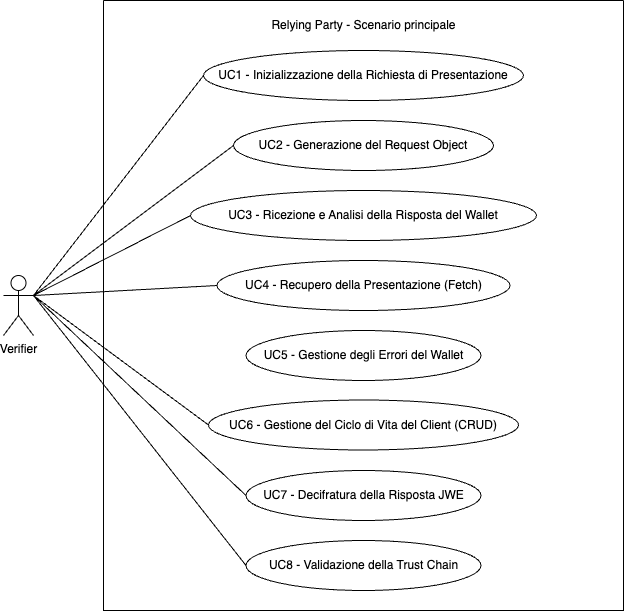
\includegraphics[width=0.7\textwidth]{./immagini/usecase/UC-Scenario Principale.png}    
    \caption{Diagramma dei casi d'uso -- Scenario principale del Relying Party}
    \label{fig:UC-Scenario Principale}
\end{figure}

\paragraph{\large\bfseries UC1: Inizializzazione della richiesta di presentazione}\mbox{}\\
\begin{figure}[H]
    \centering
    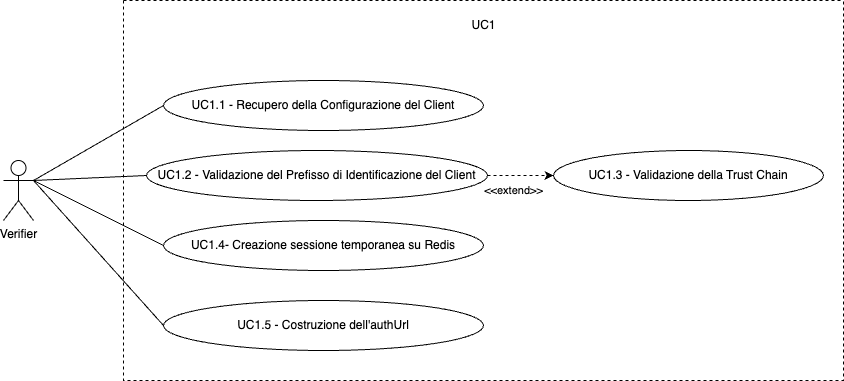
\includegraphics[width=0.7\textwidth]{./immagini/usecase/UC1.png}    
    \caption{UC1 -- Inizializzazione della richiesta di presentazione}
    \label{fig:UC1}
\end{figure}

\noindent\textbf{Attori:} Verifier, Utente finale.
\\
\textbf{Descrizione:} L'Utente finale, mediante l'interfaccia \textit{frontend} del Relying Party, avvia una nuova sessione di richiesta di presentazione di Credenziali Verificabili. Il Verifier procede alla validazione dell'identità del client precedentemente configurato, effettua — ove previsto dal \textit{Client ID Scheme} adottato — la verifica della \textit{Trust Chain} (nel caso di OpenID Federation), istanzia una sessione temporanea su Redis contenente la \textit{DCQL Query}, un \textit{nonce} crittografico e un identificativo univoco, e restituisce all'interfaccia \textit{frontend} un URL di autorizzazione (\texttt{authUrl}) e un identificativo di sessione (\texttt{sessionId}).
\\
\textbf{Precondizioni:}
\begin{itemize}
    \item Il client (Verifier) è stato precedentemente configurato nell'istanza MongoDB con parametri \texttt{redirectUris} e \texttt{vpFormatsSupported} validi.
    \item Il server Redis è raggiungibile e operativo.
    \item Le variabili d'ambiente del sistema sono configurate correttamente.
    \item Qualora il prefisso del \texttt{clientId} sia \texttt{openid\_federation}, la variabile d'ambiente \texttt{VERIFIER\_ENTITY\_IDENTIFIER} deve risultare impostata e le \textit{Trusted Authorities} devono essere raggiungibili.
    \item Qualora il prefisso sia \texttt{verifier\_attestation}, la variabile d'ambiente \texttt{VERIFIER\_ATTESTATION\_JWT} deve contenere un token JWT di attestazione valido.
\end{itemize}
\noindent\textbf{Postcondizioni:}
\begin{itemize}
    \item Una nuova sessione con stato \texttt{pending} è stata istanziata su Redis con un TTL (\textit{Time To Live}) configurato.
    \item La sessione contiene i seguenti parametri: \texttt{sessionId}, \texttt{requestId}, \texttt{nonce}, \texttt{transactionId}, \texttt{dcqlQuery}, \texttt{responseMode}, \texttt{prefixClientId}, \texttt{responseUri}.
    \item L'interfaccia \textit{frontend} ha ricevuto l'\texttt{authUrl} (contenente le informazioni necessarie al Wallet per elaborare la richiesta) e il \texttt{sessionId} (necessario per il successivo recupero della presentazione).
\end{itemize}

\noindent\textbf{Scenario principale:}
\begin{enumerate}
    \item L'Utente, mediante l'interfaccia \textit{frontend}, invia una richiesta HTTP \texttt{POST} all'endpoint \texttt{/init} con un payload contenente i parametri e \texttt{dcqlQuery}.
    \item Il Verifier recupera la configurazione del client dall'istanza MongoDB tramite i parametri \texttt{domainId} e \texttt{clientId}.
    \item Il Verifier valida il prefisso del \texttt{clientId}.
    \item Qualora il prefisso sia \texttt{openid\_federation}, il Client costruisce e valida la \textit{Trust Chain} verso il \textit{Trust Anchor} configurato.
    \item Il Verifier genera un \texttt{nonce}, un \texttt{requestId}, un \texttt{transactionId} e un \texttt{sessionId}.
    \item La sessione viene persistita su Redis.
    \item Il Verifier costruisce l'\texttt{authUrl}.
    \item Il Verifier restituisce una risposta HTTP \texttt{201 Created} con payload \texttt{\{success: true, sessionId, authUrl\}}.
\end{enumerate}

\noindent\textbf{Scenario alternativo:}
\begin{itemize}
    \item Qualora non risulti configurato alcun Verifier per il \texttt{domainId} fornito, il sistema solleva un'eccezione. Viene restituita una risposta HTTP \texttt{403 Forbidden}.
    \item Qualora il \texttt{TrustAnchorService} non riesca a costruire la \textit{Trust Chain}, il sistema solleva un'eccezione. Viene restituita una risposta HTTP \texttt{403 Forbidden}.
    \item Qualora non sia configurato l'url per il flusso \texttt{openid\_federation}, il sistema solleva un'eccezione. Viene restituita una risposta HTTP \texttt{400 Bad Request}.
    \item Qualora il prefisso fornito non sia valido, il sistema solleva un'eccezione. Viene restituita una risposta HTTP \texttt{501 Not Implemented}.
    \item Qualora il prefisso sia \texttt{verifier\_attestation} ma il token JWT non risulti valido, il sistema solleva un'eccezione. Viene restituita una risposta HTTP \texttt{400 Bad Request}.
\end{itemize}
\paragraph{\large\bfseries UC1.1: Verifica dell'identità del client configurato}
\label{uc:verifier:uc1.1}
\mbox{}\\
\noindent\textbf{Attori:} Verifier.
\\
\noindent\textbf{Descrizione:} Il Verifier recupera dall'istanza MongoDB la configurazione del client associato ai parametri \texttt{domainId} e \texttt{clientId} ricevuti nella richiesta HTTP. Tale configurazione comprende i parametri necessari per l'intero flusso di presentazione: \texttt{redirectUris}, \texttt{vpFormatsSupported}, \texttt{jwks} e gli algoritmi crittografici supportati.
\\
\noindent\textbf{Precondizioni:}
\begin{itemize}
    \item I parametri \texttt{domainId} e \texttt{clientId} sono stati forniti nella richiesta HTTP.
    \item L'istanza MongoDB è raggiungibile e operativa.
\end{itemize}
\noindent\textbf{Postcondizioni:}
\begin{itemize}
    \item L'oggetto \texttt{Client} è stato recuperato dall'istanza MongoDB.
\end{itemize}

\noindent\textbf{Scenario principale:}
\begin{enumerate}
    \item Il Verifier recupera la configurazione del client dal repository MongoDB.
    \item L'oggetto estratto dal repository viene validato e vengono verificati i campi obbligatori.
\end{enumerate}

\noindent\textbf{Scenario alternativo:}
\begin{itemize}
    \item Qualora nessun record corrisponda alla coppia \texttt{domainId}/\texttt{clientId} fornita, il sistema solleva un'eccezione e viene restituita una risposta HTTP \texttt{403 Forbidden}.
\end{itemize}

\paragraph{\large\bfseries UC1.2: Validazione del prefisso di identificazione del client}
\label{uc:verifier:uc1.2}
\mbox{}\\
\noindent\textbf{Attori:} Verifier.
\\
\noindent\textbf{Descrizione:} Il Verifier effettua il \textit{parsing} e la validazione del prefisso di identificazione del client (\texttt{prefixClientId}) al fine di determinare la modalità di autenticazione del Verifier nei confronti del Wallet.
\\
\noindent\textbf{Precondizioni:}
\begin{itemize}
    \item Il parametro \texttt{prefixClientId} è stato fornito nel corpo della richiesta HTTP; qualora risulti vuoto, viene applicato il valore predefinito \texttt{pre\_registered}.
    \item La configurazione del client è stata recuperata con successo (rif. \ref{uc:verifier:uc1.1}).
\end{itemize}
\noindent\textbf{Postcondizioni:}
\begin{itemize}
    \item Il prefisso è stato ricondotto a uno dei seguenti valori: \texttt{redirect\_uri}, \texttt{x509\_san\_dns}, \texttt{x509\_hash}, \texttt{openid\_federation}, \texttt{verifier\_attestation}, \texttt{pre\_registered}.
    \item Il risultato della validazione include i seguenti attributi: \texttt{clientIdValue}, \texttt{requiresSignature}, \texttt{headerExtensions}, \texttt{clientMetadataPolicy}.
\end{itemize}
\noindent\textbf{Scenario principale:}
\begin{enumerate}
    \item Il Verifier effettua il \textit{parsing} del valore del prefisso.
    \item In base al prefisso riconosciuto, il sistema applica la corrispondente logica di validazione:
    \begin{itemize}
        \item \texttt{redirect\_uri}: il valore \texttt{clientIdValue} viene costruito concatenando il prefisso al \texttt{responseUri} nella forma \texttt{redirect\_uri:<responseUri>}. Non è richiesta la firma crittografica del \textit{Request Object}. La politica sui metadati del client è impostata a \texttt{MUST\_INCLUDE}.
        \item \texttt{x509\_san\_dns}: dal JWKS del client viene estratta la catena certificativa \texttt{x5c} e viene validato il certificato \textit{leaf}. È richiesta la firma crittografica. La politica sui metadati è impostata a \texttt{MUST\_INCLUDE}.
        \item \texttt{x509\_hash}: dal JWKS viene estratta la catena \texttt{x5c} e viene calcolato il digest SHA-256 del certificato \textit{leaf}, utilizzato come identificativo del client. È richiesta la firma crittografica. La politica sui metadati è impostata a \texttt{MUST\_INCLUDE}.
        \item \texttt{openid\_federation}: come identificativo viene adottato il valore dell'\texttt{entityIdentifier}. È richiesta la firma crittografica. I metadati del client non devono essere inclusi nella richiesta (\texttt{MUST\_EXCLUDE}).
        \item \texttt{verifier\_attestation}: viene effettuato il \textit{parsing} del JWT di attestazione del Verifier, dal quale vengono estratti i claim \texttt{sub} e \texttt{cnf}. Il sistema verifica inoltre che il \texttt{responseUri} sia presente nella lista \texttt{redirect\_uris} contenuta nel JWT. È richiesta la firma crittografica. La politica sui metadati è impostata a \texttt{MUST\_INCLUDE}.
        \item \texttt{pre\_registered}: viene utilizzato direttamente il \texttt{clientId} già registrato nel sistema. Non è richiesta la firma crittografica. L'inclusione dei metadati è facoltativa (\texttt{NOT\_REQUIRED}).
    \end{itemize}
\end{enumerate}
\noindent\textbf{Scenario alternativo:}
\begin{itemize}
    \item Qualora il prefisso fornito sia \texttt{origin} viene restituita una risposta HTTP \texttt{501 Not Implemented}.
    \item Per i prefissi \texttt{x509\_san\_dns} e \texttt{x509\_hash}, qualora il JWKS del client non contenga una chiave di firma provvista di catena certificativa \texttt{x5c}, viene restituita una risposta HTTP \texttt{400 Bad Request}.
    \item Per il prefisso \texttt{x509\_san\_dns}, qualora nessun \texttt{dnsName} sia presente nel certificato corrisponda all'\textit{hostname} del \texttt{responseUri}, viene restituita una risposta HTTP \texttt{403 Forbidden}.
    \item Per il prefisso \texttt{verifier\_attestation}, qualora il JWT risulti privo dei claim \texttt{sub} o \texttt{cnf}, viene restituita una risposta HTTP \texttt{400 Bad Request}.
    \item Per il prefisso \texttt{verifier\_attestation}, qualora il \texttt{responseUri} non sia incluso nella lista \texttt{redirect\_uris} del JWT di attestazione, viene restituita una risposta HTTP \texttt{403 Forbidden}.
\end{itemize}

\paragraph{\large\bfseries UC1.3: Validazione della Trust Chain}
\label{uc:verifier:uc1.3}
\mbox{}\\
\noindent\textbf{Attori:} Verifier.
\\
\noindent\textbf{Descrizione:} Qualora il prefisso di identificazione del client sia \texttt{openid\_federation}, il sistema procede alla verifica della \textit{Trust Chain} dell'OpenID Provider, preliminarmente alla generazione della sessione.
\\
\noindent\textbf{Precondizioni:}
\begin{itemize}
    \item Il prefisso identificato nel caso d'uso UC1.2 (rif. \ref{uc:verifier:uc1.2}) è \texttt{openid\_federation}.
    \item La variabile d'ambiente \texttt{OPENID4VCI\_AUTHORIZE\_URL} è configurata e l'endpoint corrispondente è raggiungibile.
    \item Almeno un \textit{Trust Anchor} è specificato nel campo \texttt{trustedAuthorities} della \textit{DCQL Query}.
\end{itemize}
\noindent\textbf{Postcondizioni:}
\begin{itemize}
    \item L'appartenenza dell'OpenID Provider alla federazione di fiducia è stata confermata mediante la validazione completa della catena.
\end{itemize}
\noindent\textbf{Scenario principale:}
\begin{enumerate}
    \item Il sistema verifica la presenza della variabile d'ambiente \texttt{OPENID4VCI\_AUTHORIZE\_URL} e ne estrae l'\texttt{entityId} dell'OpenID Provider.
    \item Vengono estratte le \texttt{trustedAuthorities} dalla \textit{DCQL Query} fornita dall'interfaccia \textit{frontend}.
    \item Il Verifier avvia la costruzione e la validazione della \textit{Trust Chain} per l'\texttt{entityId} dell'OpenID Provider.
\end{enumerate}

\noindent\textbf{Scenario alternativo:}
\begin{itemize}
    \item Qualora la variabile d'ambiente non risulti configurata, viene restituita una risposta HTTP \texttt{400 Bad Request}.
    \item Qualora il \texttt{TrustAnchorService} rilevi una catena non valida, viene restituita una risposta HTTP \texttt{403 Forbidden}.
\end{itemize}

\paragraph{\large\bfseries UC1.4: Creazione della sessione temporanea su Redis}
\label{uc:verifier:uc1.4}
\mbox{}\\
\noindent\textbf{Attori:} Verifier.
\\
\noindent\textbf{Descrizione:} Il Verifier genera l'insieme degli identificativi crittografici necessari per la sessione e ne effettua la persistenza su Redis con un TTL (\textit{Time To Live}) configurabile.
\\
\noindent\textbf{Precondizioni:}
\begin{itemize}
    \item La validazione del prefisso è stata completata con successo (rif. \ref{uc:verifier:uc1.2}).
    \item Qualora il prefisso sia \texttt{openid\_federation}, la \textit{Trust Chain} è stata validata (rif. \ref{uc:verifier:uc1.3}).
    \item Il server Redis è raggiungibile e operativo.
\end{itemize}
\noindent\textbf{Postcondizioni:}
\begin{itemize}
    \item Una nuova sessione con stato \texttt{pending} è stata persistita su Redis, indicizzata mediante il \texttt{requestId} come chiave primaria.
    \item Il TTL è stato impostato.
\end{itemize}
\noindent\textbf{Scenario principale:}
\begin{enumerate}
    \item Il Verifier genera i seguenti identificativi crittografici:
    \begin{itemize}
        \item \texttt{requestId}: utilizzato come parametro \texttt{state} nel protocollo OID4VP.
        \item \texttt{nonce}: impiegato per la prevenzione degli attacchi di tipo \textit{replay}.
        \item \texttt{transactionId}: deputato al collegamento tra sessione e \textit{Response Record}.
        \item \texttt{sessionId}: restituito all'interfaccia \textit{frontend} per il successivo recupero della presentazione.
    \end{itemize}
    \item Viene istanziato l'oggetto \texttt{Session} con validazione dei campi obbligatori e verifica della conformità dei valori \texttt{nonce} e \texttt{requestId}.
    \item Il Client effettua la serializzazione dell'oggetto in formato JSON e ne esegue la persistenza su Redis con il TTL configurato.
\end{enumerate}
\noindent\textbf{Scenario alternativo:}
\begin{itemize}
    \item Qualora i valori \texttt{nonce} o \texttt{requestId} generati non superino la validazione di conformità viene restituita una risposta HTTP \texttt{400 Bad Request}.
\end{itemize}

\paragraph{\large\bfseries UC1.5: Costruzione dell'Authorization URL}\mbox{}\\
\noindent\textbf{Attori:} Verifier.
\\
\noindent\textbf{Descrizione:} Il Verifier costruisce l'URL di autorizzazione (\texttt{authUrl}) destinato a essere restituito all'interfaccia \textit{frontend} e successivamente presentato al Wallet mediante codice QR o \textit{deep link}.
\\
\noindent\textbf{Precondizioni:}
\begin{itemize}
    \item La sessione è stata creata con successo (rif.\ \ref{uc:verifier:uc1.4}).
    \item Il risultato della validazione del prefisso è disponibile (rif.\ \ref{uc:verifier:uc1.2}).
\end{itemize}
\noindent\textbf{Postcondizioni:}
\begin{itemize}
    \item L'\texttt{authUrl} è stato costruito nel formato conforme al tipo di prefisso adottato.
\end{itemize}
\noindent\textbf{Scenario principale:}
\begin{enumerate}
    \item Qualora la firma crittografica non sia richiesta: l'URL viene costruito utilizzando i seguenti \textit{query parameters}: \texttt{client\_id}, \texttt{response\_type=vp\_token}, \texttt{response\_mode}, \texttt{response\_uri}, \texttt{nonce}, \texttt{state} (corrispondente al \texttt{requestId}) e \texttt{dcql\_query}. Qualora la \texttt{clientMetadataPolicy} sia impostata a \texttt{MUST\_INCLUDE}, viene aggiunto il parametro \texttt{client\_metadata} contenente \texttt{vpFormatsSupported} e, opzionalmente, \texttt{jwks}.
    \item Qualora la firma crittografica sia richiesta: l'URL viene costruito includendo esclusivamente i parametri \texttt{client\_id}, \texttt{request\_uri} (puntante all'endpoint \texttt{/request/:requestId}) e \texttt{request\_uri\_method=post}.
\end{enumerate}

\section{Limiti}

\chapter{Progettazione}
\label{cap:progettazione}
In questo capitolo verrà trattato il secondo periodo del tirocinio: la progettazione e la codifica. Questa parte, avvenuta dopo l'Analisi dei Requisiti, è da ritenersi importante per il progetto in quanto ha occupato gran parte del tempo lavorativo. Il primo passo è stato eseguire la progettazione dell'architettura, in modo che i servizi necessari fossero correttamente configurati prima del loro effettivo utilizzo. Successivamente è stata eseguita la stesura del codice per la realizzazione della Skill. Nei paragrafi successivi seguiranno porzioni di codice significativo per la loro importanza e per il funzionamento di determinati servizi. Importante ricordare che il codice implementato e mostrato sarà in Node.js come quanto detto nel paragrafo \hyperref[nodejs]{1.4.1}. 

\section{Architettura}
Come riportato nel paragrafo \hyperref[serivizi-aws]{1.4.3}, il progetto si basa interamente sui servizi offerti dall'ecosistema Amazon. Di conseguenza è risultato facile ed immediato impostare i servizi dell'architettura in modo da rendere il tutto efficacie ed efficiente. In questo paragrafo si andrà a spiegare cosa offre ogni singolo servizio di AWS e come esso è stato impostato per il suo corretto funzionamento nella Skill.

\chapter{Codifica}
\label{cap:codifica}
Dopo aver completato la fase di progettazione è stata eseguita la fase di codifica e validazione. Questo capitolo sarà il conseguimento della seconda parte del periodo di stage dove verranno spiegate le funzionalità implementate nella Skill mostrando porzioni di codice. Verrà inoltro spiegata la struttura del progetto: le varie cartelle contenti i file delle \textit{classi} realizzate e i \textit{packages} installati. 

\section{Organizzazione del codice}
Successivamente alla parte di comprensione e configurazione dei servizi utilizzati in questo progetto, e alla creazione della Skill, è stato eseguito un micro-processo di organizzazione del codice prima della sua stesura. Questa pratica adottata è stata necessaria per avere uno schema e una gerarchia delle parti di codice che sono state sviluppate durante il periodo di tirocinio. Tale organizzazione ha permesso di sviluppare in maniera più ordinata e consapevole riducendo la probabilità di introdurre errori e rendendo il codice più manutenibile. Pertanto la cartella del progetto è stata così disposta:
\chapter{Verifica e validazione}
\label{cap:verifica_validazione}
L'ultima fase del periodo di tirocinio ha riguardato il processo di verifica e validazione. La prima è un processo che si occupa di fornire evidenza oggettiva, ovvero che i risultati ottenuti come output dello sviluppo del software soddisfino i requisiti, la seconda invece è un processo per confermare in modo definitivo che le caratteristiche del software siano conformi ai bisogni dell'utente e all'uso previsto.
Per eseguire la verifica e la validazione è necessario l'esecuzione di test\footnote{In ambito informatico i test eseguiti nel processo di verifica sono eseguiti in maniera automatica durante lo sviluppo del software} che individuino carenze, correttezza e affidabilità. Nel progetto della Skill Concierge Croccante non è stato realizzato alcun test per il processo di verifica: viste le tempistiche non è stato potuto fare ciò e si è pertanto scelto di eseguire test già esistenti nel servizio Amazon Lambda, sufficienti ad esaminare il codice e rilevare eventuali errori. Per quanto riguarda il processo di validazione\footnote{Attività di supporto la quale accerta che il prodotto dei processi rispetti le specifiche} è stato svolto, alla fine del periodo di tirocinio, un incontro  con il tutor aziendale e CFO Damiano Buscemi come conferma fiale la quale ha accertato le bontà richieste dal prodotto finale. Tale validazione non è stata altro che una dimostrazione funzionante della Skill, eseguita prima da me per spiegare le varie funzionalità, ed infine da Crispy Bacon come conferma.
\chapter{Valutazione finale}
\label{cap:valutazione_finale}

\section{Obiettivi raggiunti}
Il progetto ha raggiunto i seguenti obiettivi primari:

\begin{itemize}
    \item \textbf{Implementazione completa del protocollo OID4VP\glsadd{oid4vpg}\glsfirstoccur{}:} il sistema supporta l'intero ciclo di vita delle \textit{Verifiable Presentations}, dalla richiesta iniziale fino al ritiro dei dati verificati, coprendo le quattro fasi previste dalla specifica.
    \item \textbf{Supporto a sei schemi di identificazione del client:} il sistema gestisce correttamente \texttt{redirect\_uri}, \texttt{x509\_san\_dns}, \texttt{x509\_hash}, \texttt{openid\_federation}, \texttt{verifier\_attestation} e \texttt{pre\_registered}, coprendo la quasi totalità degli scenari previsti dal draft OID4VP\glsadd{oid4vpg}.
    \item \textbf{Verifica crittografica SD-JWT\glsadd{sdjwtg}\glsfirstoccur{} end-to-end:} il sistema è in grado di analizzare, validare gli hash delle \textit{disclosure}, verificare la firma dell'Issuer e convalidare il \textit{Key Binding JWT\glsadd{jwtg}\glsfirstoccur{}}, garantendo sia l'autenticità sia la titolarità delle credenziali.
    \item \textbf{Risoluzione ricorsiva delle Trust Chain\glsadd{trustchaing}\glsfirstoccur{}:} l'algoritmo DFS\glsadd{dfs}\glsfirstoccur{} implementato nel \texttt{TrustAnchorService} è in grado di risolvere catene di fiducia arbitrariamente profonde con protezione contro i cicli.
    \item \textbf{Sicurezza Forward Secrecy\glsadd{forwardsecrecyg}\glsfirstoccur{}:} il meccanismo di chiavi effimere con distruzione atomica tramite \texttt{GETDEL} garantisce che la compromissione di una chiave non comprometta sessioni passate.
    \item \textbf{Multi-tenancy\glsadd{multitenancyg}\glsfirstoccur{} nativo:} l'isolamento dei dati per dominio è garantito sia a livello applicativo sia a livello di database, mediante indici composti su MongoDB.
    \item \textbf{Superamento dei Conformance Test OID4VP\glsadd{oid4vpg}:} il sistema ha superato con successo i test di conformità ufficiali della OpenID Foundation per il profilo Verifier, come descritto nel Capitolo~\ref{cap:verifica_validazione}, certificando l'interoperabilità e la correttezza del comportamento di protocollo.
\end{itemize}

\section{Debito tecnico e limiti}
È necessario riconoscere con rigore i limiti del lavoro svolto, che costituiscono il debito tecnico del progetto:

\begin{enumerate}
    \item \textbf{Assenza di test automatizzati.} Il progetto non include test unitari, di integrazione né end-to-end. Non è installato alcun framework di testing (Jest, Vitest, Mocha), nonostante la presenza di \texttt{ioredis-mock} nelle \texttt{devDependencies} e la riga commentata \texttt{\# RUN yarn test} nel \texttt{Dockerfile} suggeriscano che il testing fosse previsto. Questa rappresenta la criticità più rilevante: la verifica dinamica dipende interamente dal testing manuale, intrinsecamente non ripetibile e non scalabile, e non è possibile integrare la verifica in una pipeline CI/CD\glsadd{cicdg}\glsfirstoccur{} con gate automatici.
    \item \textbf{Curva EC limitata a P-256.} L'\texttt{EphemeralKeyService} genera sempre chiavi effimere con curva P-256, indipendentemente dall'algoritmo JWE\glsadd{jweg}\glsfirstoccur{} negoziato. Algoritmi come \texttt{ECDH-ES+A256KW} (che beneficerebbe di P-384 o P-521) e lo scambio basato su X25519 non sono pertanto supportati.
    \item \textbf{Disclosure di tipo array non supportate.} Il \texttt{SdJwtCredentialVerifierService} gestisce esclusivamente le \textit{disclosure} a tre elementi (salt, nome del claim, valore). Le \textit{disclosure} a due elementi (salt, valore), utilizzate per elementi all'interno di array, producono esplicitamente un errore. Questo limita la capacità del sistema di gestire credenziali SD-JWT\glsadd{sdjwtg} con claim a valori multipli.
    \item \textbf{Assenza di caching per le Entity Configuration.} Ogni invocazione del \texttt{TrustAnchorService} per la validazione di una Trust Chain\glsadd{trustchaing} esegue chiamate HTTP\glsadd{http}\glsfirstoccur{} verso gli endpoint \texttt{/.well-known/openid-federation} senza alcun meccanismo di cache. In scenari con molteplici richieste per il medesimo Issuer, questo genera traffico di rete ridondante e latenza evitabile.
    \item \textbf{Verifica della firma dell'Attestation JWT\glsadd{jwtg} mancante.} Nel metodo \texttt{validateVerifierAttestation} del \texttt{ClientIdPrefixValidator}, il JWT\glsadd{jwtg} di attestazione viene decodificato per estrarne i claim, ma la firma non viene verificata crittograficamente contro la chiave pubblica dell'autorità emittente.
    \item \textbf{Copertura parziale dei formati di credenziali.} I Conformance Test eseguiti hanno coperto il formato \texttt{dc+sd-jwt}, ma il sistema dichiara di poter supportare anche il formato \texttt{mso\_mdoc} (ISO 18013-5) tramite la struttura \texttt{MdocFormatSupported} nel modello \texttt{Client}. Nessun servizio di verifica per questo formato è stato implementato, e la discrepanza tra le capacità dichiarate e quelle testate costituisce un rischio di conformità.
    \item \textbf{Assenza di test di performance e carico.} Non sono stati condotti test di performance, load testing o stress testing. L'assenza di dati sulle performance sotto carico (latenza media, throughput, comportamento sotto contention su Redis) rappresenta un'incognita per il dimensionamento dell'infrastruttura in scenari di produzione.
    \item \textbf{Validazione limitata ai flussi di protocollo.} I Conformance Test validano la conformità del protocollo dall'esterno, ma non entrano nel merito della correttezza interna dell'implementazione: non verificano, ad esempio, che la chiave privata effimera venga effettivamente distrutta dopo l'uso (\textit{Forward Secrecy}\glsadd{forwardsecrecyg}), che il consumo della sessione sia realmente atomico sotto concorrenza, o che il convertitore di nomenclatura non corrompa strutture dati con chiavi non previste.
\end{enumerate}

\section{Sviluppi futuri e miglioramenti proposti}
Sulla base dell'analisi dei limiti, i principali assi di miglioramento per le iterazioni successive sono:

\begin{itemize}
    \item \textbf{Introduzione di una suite di test completa:} installazione di Jest o Vitest, scrittura di test unitari per i servizi di validazione crittografica (utilizzando \texttt{ioredis-mock} per Redis) e test di integrazione per i flussi end-to-end. La priorità dovrebbe essere assegnata ai servizi \texttt{trust-anchor.service.ts}, \texttt{credential-verifier.service.ts} e \texttt{prefix-validator.service.ts}, dove un errore è più critico.
    \item \textbf{Integrazione nella pipeline CI/CD\glsadd{cicdg}:} decommentare la riga \texttt{RUN yarn test} nel \texttt{Dockerfile} e configurare una pipeline di CI/CD (ad esempio GitLab CI o GitHub Actions) che esegua automaticamente \texttt{yarn typecheck}, \texttt{yarn lint}, \texttt{yarn test} e \texttt{yarn audit} ad ogni commit, bloccando il merge in caso di fallimento.
    \item \textbf{Test di integrazione end-to-end e di concorrenza:} scrittura di test che simulino l'intero flusso delle quattro fasi OID4VP\glsadd{oid4vpg} in un ambiente controllato, verificando le transizioni di stato, la generazione e distruzione delle chiavi effimere, e la correttezza dei payload. Inoltre, test specifici che invochino \texttt{consumeSessionForResponse()} e \texttt{retrieveAndDestroyPrivateKey()} in modo concorrente per verificare che l'atomicità sia garantita sotto contention.
    \item \textbf{Supporto a curve EC multiple e X25519:} parametrizzazione della curva EC nell'\texttt{EphemeralKeyService} in base all'algoritmo JWE\glsadd{jweg} negoziato, con supporto a P-384, P-521 e, in prospettiva, X25519 per lo scambio chiavi Diffie-Hellman.
    \item \textbf{Implementazione delle array \textit{disclosure}:} completamento del supporto a \textit{disclosure} a due elementi nel \texttt{SdJwtCredentialVerifierService}, abilitando la verifica di credenziali SD-JWT\glsadd{sdjwtg} con claim a valori multipli.
    \item \textbf{Implementazione di un layer di caching per le Entity Configuration:} salvataggio in Redis (con TTL\glsadd{ttlg}\glsfirstoccur{} basato sul claim \texttt{exp}) delle \textit{Entity Configuration} e dei \textit{Subordinate Statement} recuperati durante la risoluzione delle Trust Chain\glsadd{trustchaing}, al fine di ridurre la latenza e il traffico di rete.
    \item \textbf{Verifica crittografica completa dell'Attestation JWT\glsadd{jwtg}:} implementazione della verifica della firma nel metodo \texttt{validateVerifierAttestation}, importando la chiave pubblica dell'autorità emittente e validando il JWT\glsadd{jwtg} con \texttt{jose.jwtVerify()}.
    \item \textbf{Estensione dei Conformance Test:} una volta implementato il supporto al formato mDoc, eseguire i Conformance Test OIDF anche per questo formato. Valutare inoltre l'esecuzione dei test per il profilo HAIP\glsadd{haipg}\glsfirstoccur{} (\textit{High Assurance Interoperability Profile}), che include requisiti aggiuntivi di sicurezza rilevanti per il contesto EUDI.
    \item \textbf{Rafforzamento della configurazione TypeScript:} l'attivazione di \texttt{strictNullChecks} (o dell'intero \texttt{strict: true}) forzerebbe il compilatore a segnalare staticamente tutti i punti in cui un valore potrebbe essere null, eliminando un'intera categoria di errori a runtime.
\end{itemize}
\appendix

\backmatter
\cleardoublepage
\chapter{Sitografia}

\nocite{*}
\printbibliography[heading=subbibliography,type=online]


\end{document}
